%!  pour pdfLatex
\documentclass[a4paper]{article}
%\usepackage[hmargin={1.5cm,1.5cm},vmargin={2.4cm,2.4cm},headheight=13.1pt]{geometry}
\usepackage[a4paper,landscape,twocolumn,
            hmargin=1.8cm,vmargin=2.2cm,headheight=13.1pt]{geometry}

\usepackage[pdftex]{graphicx,color}
\usepackage[pdftex,colorlinks={true},urlcolor={blue},pdfauthor={remy Nicolai}]{hyperref}

\usepackage[T1]{fontenc}
\usepackage[utf8]{inputenc}

\usepackage{lmodern}
\usepackage[frenchb]{babel}

\usepackage{fancyhdr}
\pagestyle{fancy}

\usepackage{floatflt}
\usepackage{maths}

\usepackage{parcolumns}
\setlength{\parindent}{0pt}

\usepackage{caption}
\usepackage{subcaption}

\usepackage{makeidx}

\usepackage[french,ruled,vlined]{algorithm2e}
\SetKwComment{Comment}{\#}{}
\SetKwFor{Tq}{tant que}{}{}
\SetKwFor{Pour}{pour}{}{}
\DontPrintSemicolon
\SetAlgoLined

\usepackage{listings}
\lstset{language=Python,frame=single}
\lstset{literate=
  {á}{{\'a}}1 {é}{{\'e}}1 {í}{{\'i}}1 {ó}{{\'o}}1 {ú}{{\'u}}1
  {Á}{{\'A}}1 {É}{{\'E}}1 {Í}{{\'I}}1 {Ó}{{\'O}}1 {Ú}{{\'U}}1
  {à}{{\`a}}1 {è}{{\`e}}1 {ì}{{\`i}}1 {ò}{{\`o}}1 {ù}{{\`u}}1
  {À}{{\`A}}1 {È}{{\'E}}1 {Ì}{{\`I}}1 {Ò}{{\`O}}1 {Ù}{{\`U}}1
  {ä}{{\"a}}1 {ë}{{\"e}}1 {ï}{{\"i}}1 {ö}{{\"o}}1 {ü}{{\"u}}1
  {Ä}{{\"A}}1 {Ë}{{\"E}}1 {Ï}{{\"I}}1 {Ö}{{\"O}}1 {Ü}{{\"U}}1
  {â}{{\^a}}1 {ê}{{\^e}}1 {î}{{\^i}}1 {ô}{{\^o}}1 {û}{{\^u}}1
  {Â}{{\^A}}1 {Ê}{{\^E}}1 {Î}{{\^I}}1 {Ô}{{\^O}}1 {Û}{{\^U}}1
  {œ}{{\oe}}1 {Œ}{{\OE}}1 {æ}{{\ae}}1 {Æ}{{\AE}}1 {ß}{{\ss}}1
  {ű}{{\H{u}}}1 {Ű}{{\H{U}}}1 {ő}{{\H{o}}}1 {Ő}{{\H{O}}}1
  {ç}{{\c c}}1 {Ç}{{\c C}}1 {ø}{{\o}}1 {å}{{\r a}}1 {Å}{{\r A}}1
  {€}{{\euro}}1 {£}{{\pounds}}1 {«}{{\guillemotleft}}1
  {»}{{\guillemotright}}1 {ñ}{{\~n}}1 {Ñ}{{\~N}}1 {¿}{{?`}}1
}

%pr{\'e}sentation des compteurs de section, ...
\makeatletter
\renewcommand{\thesection}{\Roman{section}.}
\renewcommand{\thesubsection}{\arabic{subsection}.}
\renewcommand{\thesubsubsection}{\arabic{subsubsection}.}
\renewcommand{\labelenumii}{\theenumii.}
\makeatother


\newtheorem*{thm}{Théorème}
\newtheorem{thmn}{Théorème}
\newtheorem*{prop}{Proposition}
\newtheorem{propn}{Proposition}
\newtheorem*{pa}{Présentation axiomatique}
\newtheorem*{propdef}{Proposition - Définition}
\newtheorem*{lem}{Lemme}
\newtheorem{lemn}{Lemme}

\theoremstyle{definition}
\newtheorem*{defi}{Définition}
\newtheorem*{nota}{Notation}
\newtheorem*{exple}{Exemple}
\newtheorem*{exples}{Exemples}


\newenvironment{demo}{\renewcommand{\proofname}{Preuve}\begin{proof}}{\end{proof}}
%\renewcommand{\proofname}{Preuve} doit etre après le begin{document} pour fonctionner

\theoremstyle{remark}
\newtheorem*{rem}{Remarque}
\newtheorem*{rems}{Remarques}

%\usepackage{maths}
%\newcommand{\dbf}{\leftrightarrows}

%En tete et pied de page
\lhead{Informatique}
%\chead{Introduction aux systèmes informatiques}
\rhead{MPSI B Hoche}
\lfoot{\tiny{Cette création est mise à disposition selon le Contrat\\ Paternité-Partage des Conditions Initiales à l'Identique 2.0 France\\ disponible en ligne http://creativecommons.org/licenses/by-sa/2.0/fr/  
} 
\rfoot{\tiny{Rémy Nicolai \jobname \; \today } }
}
\makeindex


\usepackage{parcolumns}
\setlength{\parindent}{0pt}

 \begin{document}
\lhead{cours IPT}
\chead{cours 1: Introduction à l'utilisation de Python le 12/09 2016}
Python est un langage de programmation\footnote{c'est un langage interprété et non compilé} qui peut être utilisé de deux manières: 
\emph{interactivement} c'est à dire en écrivant une instruction (ou plusieurs) dans un interpréteur puis en l'exécutant immédiatement ou bien en écrivant (avec un éditeur) un fichier texte enregistré (\emph{extension} .py) ce qui permet de le conserver et de l'exécuter de manière différée.\newline
Sous diverses réserves (en particulier des problèmes de \emph{chemins de dossier} peuvent se produire), cela peut se faire dans n'importe quelle console\footnote{une console est une application dont l'interface avec l'utilisateur est uniquement du texte (ligne de commande).}. Toutefois le programme officiel de la classe nous demande d'utiliser Python par l'intermédiaire d'un \emph{environnement de programation}; les machines des salles de TP du lycée sont équipées de Spyder.\newline
L'objectif de ce cours est de se familiariser avec la notion d'environnement de travail et avec les premiers principes de Python.

\section{Environnement}
Un environnement de travail est constitué de plusieurs fenêtres (Figure \ref{fig:spyder}) qui doivent permettre les deux modes d'utilisation. Les environnements évolués comme Spyder offrent d'autres fonctionalités\footnote{par exemple des outils de vérification (débogage).}.
\begin{itemize}
 \item Dans une fenêtre console/interpréteur, on peut écrire directement une intruction Python et l'exécuter en tapant "Entrée". 
 \item Dans la fenêtre "Editeur de texte" on peut écrire, enregistrer, ... des fichiers d'extension \verb|.py| puis les faire exécuter (bouton Executer du menu ou flèche verte (suivant les versions)) dans une fenêtre console/interpréteur)
\end{itemize}
 
 \begin{figure}[h!]
 \centering
 %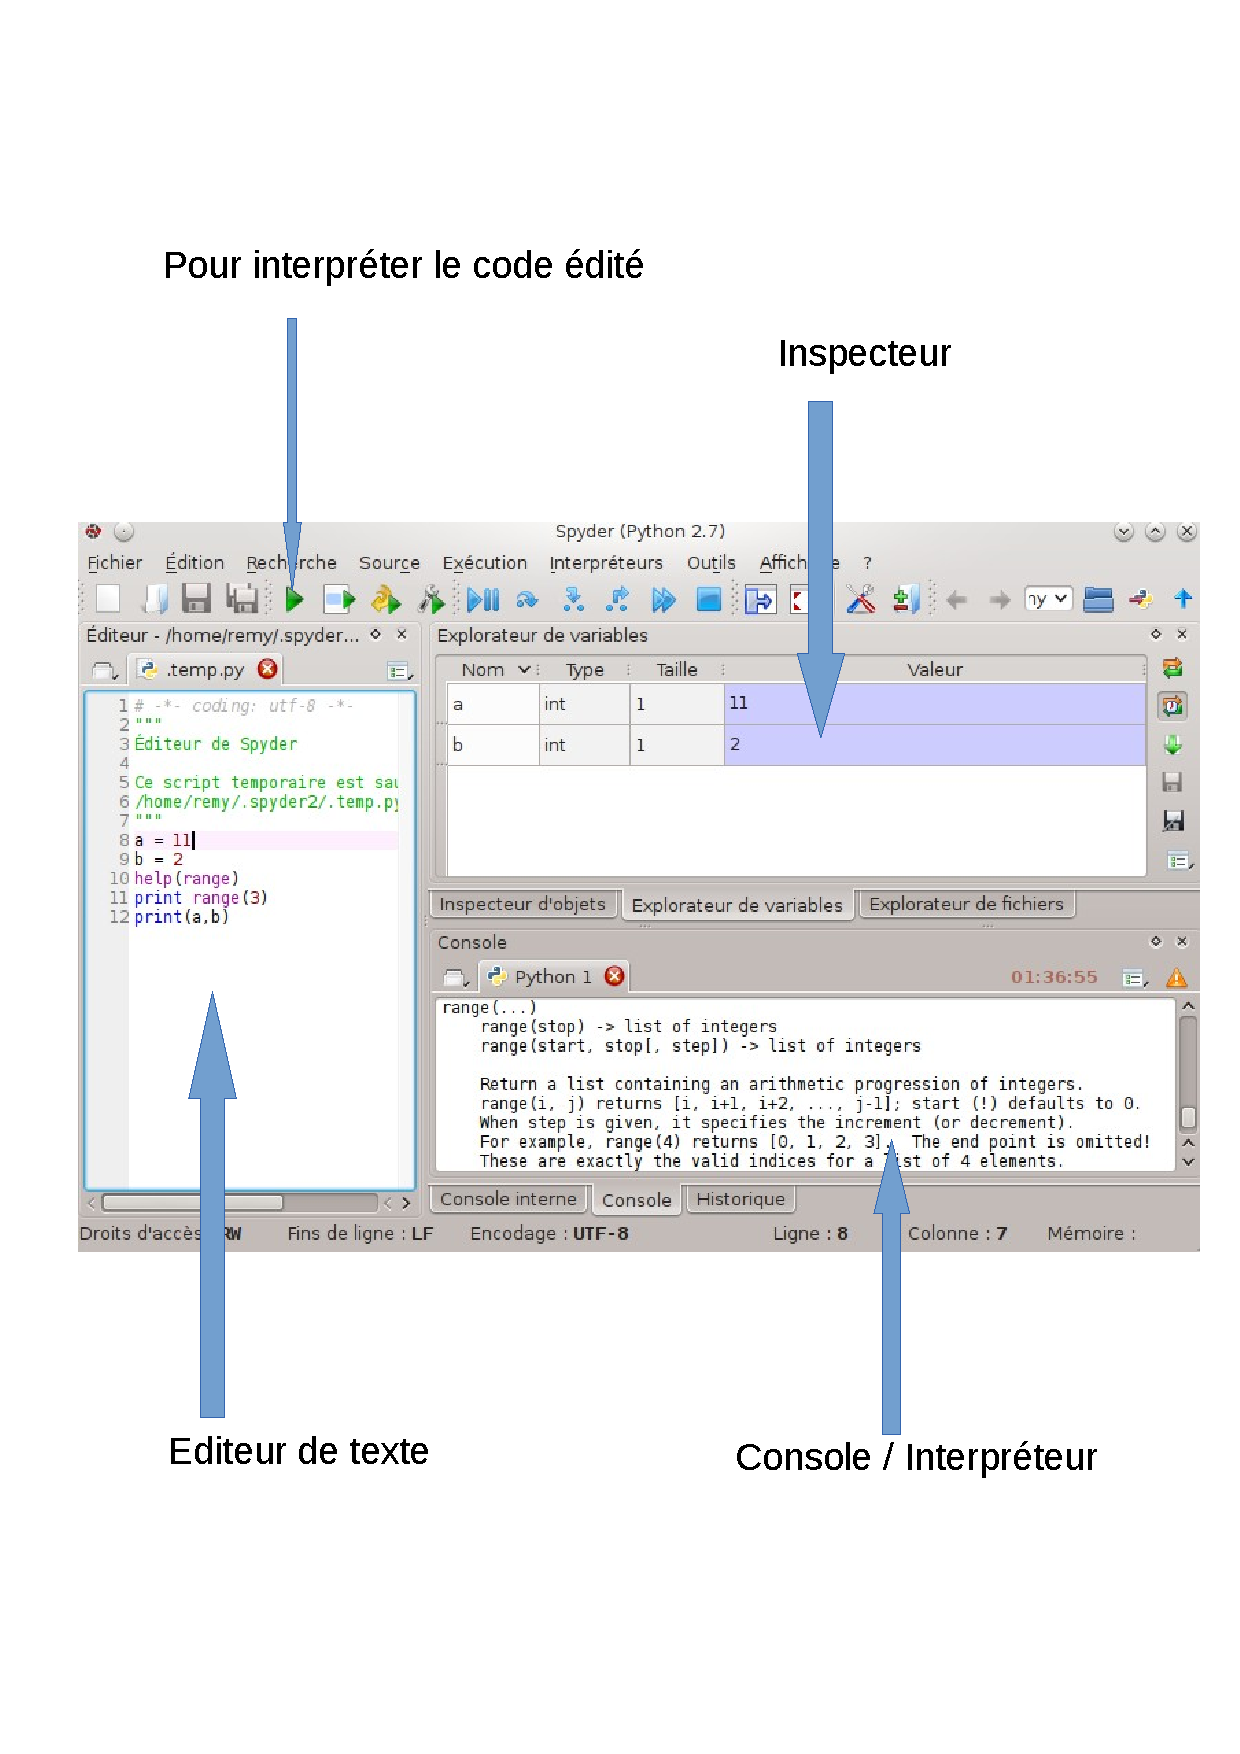
\includegraphics[width=10cm,keepaspectratio=true]{./spyder.pdf}
 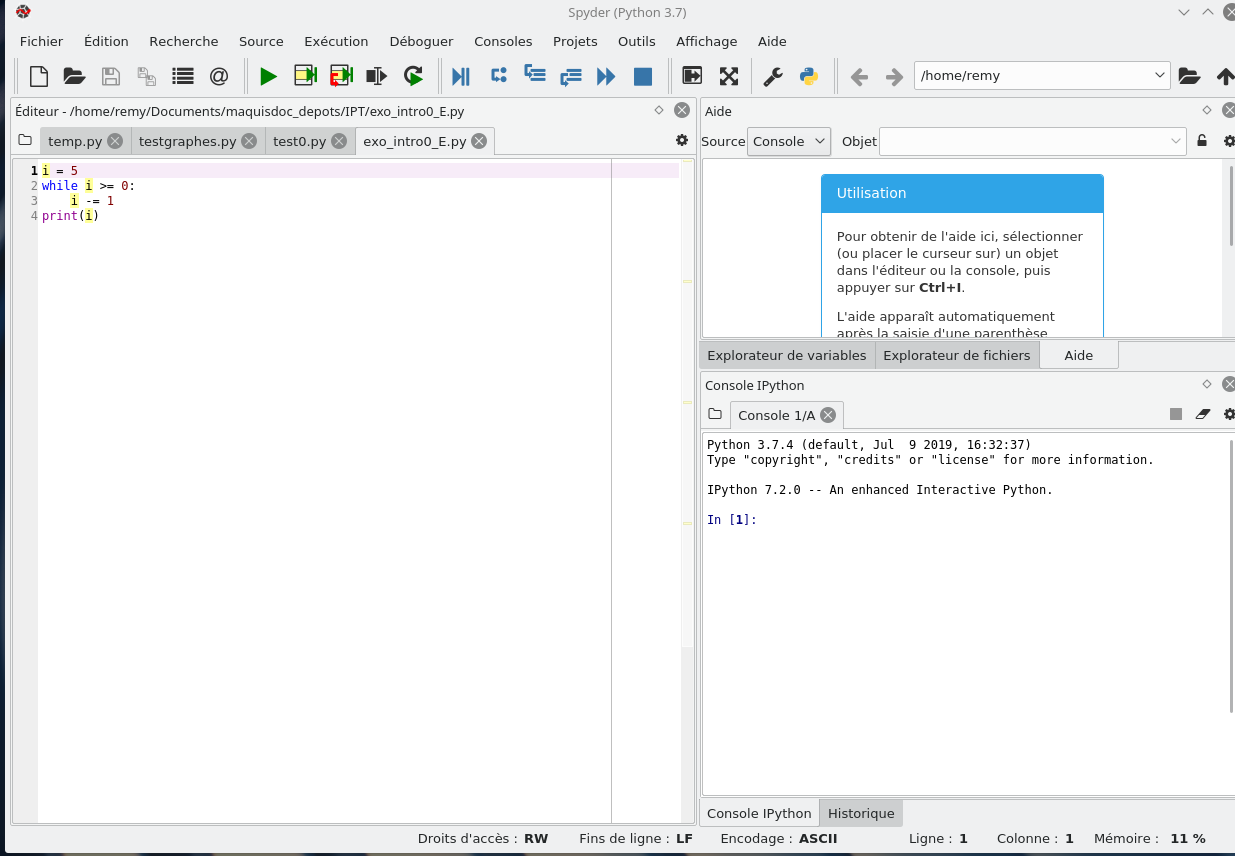
\includegraphics[width=10cm]{environnement_1.png}
 % spyder.pdf: 595x842 pixel, 72dpi, 20.99x29.70 cm, bb=0 0 595 842
 \caption{Environnement de développement spyder}
 \label{fig:spyder}
\end{figure}


Exemple avec les instructions \texttt{1+1} et \texttt{print "coucou"} ou \texttt{print("coucou")} à interpréter directement ou à exécuter par l'intermédiaire d'un fichier. Lors de l'utilisation d'un fichier, bien maitriser sa place dans l'arborescence des disques.

Il arrive souvent que le code soit mal écrit et conduise à un processus qui ne s'arrête jamais (boucle infinie). Il faut savoir comment l'arrêter.
Par exemple
 \begin{verbatim}
i = 0
while 0 < 10:
    print('coucou'+str(i))
    i+=1
 \end{verbatim}
\emph{Bien respecter l'indentation} c'est à dire les espaces en début de ligne. Faites interpréter ce code avec avec la flèche verte (dans Spyder). Comme on a formé délibérément une \emph{boucle infinie} \index{boucle infinie}, il faut pouvoir forcer l'arrêt de l'interpréteur. La fenêtre de l'interpréteur contient en principe un bouton permettant de le faire. En général ce bouton est placé en haut à droite de la ligne de menu. Sa forme dépend de l'environnement: petit triangle jaune avec un point d'exclamation, carré rouge, ....
On peut citer d'autres environnements, notamment des interpréteurs en ligne: par exemple \href{http://shell.appspot.com}{shell.appspot.com} ou \href{http://live.sympy.org/shellmobile}{live.sympy.org/shellmobile} qui est adapté aux écrans de smartphone et orienté calcul formel  (utilisant le module sympy). 

%\clearpage

\section{Exemples d'instructions}
Diverses instructions sont proposées dans la colonne de gauche. On se propose de les faire interpréter et de comprendre ce qui est renvoyé à l'aide des commentaires fournis dans la colonne de droite.
\begin{parcolumns}[rulebetween,distance=1cm,colwidths={1= .35\linewidth}]{2}
  \colchunk{\texttt{128, id(128), type(128)}}
  \colchunk{\texttt{128} est l'expression littérale \index{littéral} du nombre $128$ et \texttt{id(128)} renvoie l'identifiant unique de cet objet dans la mémoire de l'interpréteur, \texttt{type(128)} renvoie son type.}
  \colplacechunks
  
  \colchunk{
  \begin{verbatim}
   5 ** 5
   5 ** 200
  \end{verbatim}
  }
  \colchunk{Les entiers ne sont pas limités. En Python 2.7, le "L" à la fin signifie que le résultat est un entier "long" c'est à dire trop grand pour être représenté par un mot machine. Python sait gérer ces entiers; en cas d'opération dans laquelle intervient un entier long, le résultat est toujours un entier long. En Python 3, on peut dire pour simplifier que tous les entiers sont longs et le marqueur "L" n'est plus utilisé}
  \colplacechunks
  
  \colchunk{
  \begin{verbatim}
   14 // 3
   14 % 3
   14.1 / 3.0
  \end{verbatim}
  }
  \colchunk{Dans une division euclidienne, le quotient est obtenu par //, le reste par \%.\newline
  En Python 2 le / entre deux entiers calcule le quotient entier de la division euclidienne alors qu'en Python 3 il calcule une valeur approchée (float: nombres en virgule flottante) du quotient rationnel.\newline
  Bonne pratique: réserver le / à une division entre nombres en virgule flottante. Bien noter que les opérations entre entiers en virgule flottante sont toujours approchées.}
  \colplacechunks
  
  \colchunk{
  \begin{verbatim}
   pi
   sin(pi)
  \end{verbatim}
  }
  \colchunk{Python n'est pas spécialement orienté vers les maths. $\pi$ n'est pas un décimal, $\sin$ est inconnu.}
  \colplacechunks
\end{parcolumns}

\begin{parcolumns}[rulebetween,distance=1cm,colwidths={1= .35\linewidth}]{2}
  \colchunk{
  \begin{verbatim}
   from math import sin
   sin(pi)
   cos(3.1)
   from math import *
   cos(3.1)
  \end{verbatim}
  }
  \colchunk{Si on veut utiliser des opérations mathématiques, on doit les importer de la bibliothèque mathématique. Le "*" permet de tout importer ce qui n'est pas une bonne pratique. Il vaut mieux garder l'espace de nommage aussi petit que possible. Noter que le nom du module est \texttt{math} sans \og s\fg.}
  \colplacechunks
  
  \colchunk{
  \begin{verbatim}
   type(42)
   type(4.2)
   type(5 ** 20)
  \end{verbatim}
  }
  \colchunk{Les entiers et les nombres en virgule flottante sont des types élémentaires de valeurs pour le langage Python}
  \colplacechunks
  
  \colchunk{
  \begin{verbatim}
    i = 1.0j
    c = i ** 2
    i, c
    type(i), type(c)
  \end{verbatim}
  }
  \colchunk{Python connait les nombres complexes. La première ligne contient une expression littérale complexe.
  }
  \colplacechunks
 
  \colchunk{
  \begin{verbatim}
   help(floor)
   int(3.2)
   int(-3.2)
   help(int)
   int("abc",16)
  \end{verbatim}
  }
  \colchunk{On peut trouver de l'aide sur une fonction dont on connait le nom en utilisant la fonction \verb|help|. Que font les fonctions \verb|ceil| ou \verb|round| ? Que renvoie la fonction \verb|int|? Les valeurs renvoyées par \verb|int(3.5)| et \verb|round(3.5)| sont-elles les mêmes pour Python?}
  \colplacechunks
\end{parcolumns}

Pour insérer un \emph{commentaire} c'est à dire une ligne qui est ignorée par l'interpréteur et ne sert qu'à aider le programmeur, il suffit de la faire commencer par un dièse \#. Pour insérer des commentaires sur plusieurs lignes, il faut les encadrer par deux lignes contenant seulement  """.


\section{Objets, Noms, Assignations}
\subsection{Principes}
En Python\footnote{ce paragraphe est tiré de du paragraphe "Data model" de la documentation officielle du projet Python.} le concept d'\emph{objet} englobe tous les types de données. 
Chaque objet a un \emph{identifiant}, un \emph{type} et une \emph{valeur}.\newline
Une fois qu'un objet est créé, son identifiant ne change jamais; on peut le voir comme \emph{l'adresse} de l'objet dans la mémoire.\footnote{L'\emph{opérateur} \texttt{is} compare les identifiants de deux objets, la \emph{fonction} \texttt{id()} renvoie un nombre représentant son identité.}\newline
Le type d'un objet est aussi fixé une fois que l'objet est créé.\footnote{On peut dire qu'un objet est une \emph{instance} de son type. Une création (construction) est une instanciation de type (classe).} Ce type détermine les opérations que l'objet supporte (ex.: a-t-il une longueur?) et les valeurs qu'il peut prendre. Les types d'objets Python comprennent en particulier diverses sortes de nombres, chaîne de caractères, \emph{tuple}, liste, dictionnaire.\newline
Suivant son type, un objet peut être \emph{modifiable} ou \emph{non-modifiable}\footnote{mutable immutable}. Cela correspond bien au sens courant du mot objet: un objet du type \texttt{thermos} est modifiable, le même objet peut contenir plus ou moins de café. En revanche l'objet \texttt{nombre entier 2} ~n'est pas modifiable. En Python les types numériques ou le type chaîne de caractère ne sont pas modifiables alors que le type liste est modifiable.\newline
Les objets ne sont jamais explicitement détruits\footnote{contrairement à d'autres langage par exemple \texttt{C}.}; dès qu'il devient impossible de les atteindre, un dispositif de \emph{ramasse-miettes}\footnote{garbage collector} se charge de le détruire pour libérer des ressources.\newline
L'accès à un objet ne se fait pas à l'aide de son identifiant mais à partir d'un \emph{nom}. L'opération de nommage qui consiste essentiellement à écrire quelque part sur un registre une association entre un nom et un identifiant (analogue en cela au passage en mairie pour une déclaration de naissance) s'appelle une \emph{assignation}.\newline 
La \emph{syntaxe} d'une assignation est de la forme suivante:
\begin{verbatim}
  nono = 1+1
\end{verbatim}
ce qui est à gauche de l'égalité est un \emph{nom}, ce qui est à droite est une \emph{expression}. L'exécution d'une telle instruction revient à
\begin{itemize}
  \item évaluer l'expression de droite à un certain objet
  \item écrire quelque part dans un registre que le nom à gauche désigne cet objet.
\end{itemize}
Le même objet peut très bien avoir plusieurs noms lorsqu'il est le résultat de l'évaluation à droite de plusieurs assignations (on parle alors d'\emph{alias} pour cet objet). En revanche un nom désigne un seul objet. Si un nom est réassigné à un nouvel objet, il est possible que l'objet qu'il désignait avant la réassignation n'ait plus de nom et soit donc inaccessible. Le travail du ramasse miette consiste à examiner le registre pour savoir si c'est le cas et éventuellement libérer de la mémoire.\newline 
En programation Python, la terminologie \og assignation\fg et \og nom\fg est préférable à \og égalité\fg et \og variable\fg.

\subsection{\'Echange de noms}
Dans certains langages, ce qui est à gauche d'un signe \texttt{=} doit être vu comme une sorte de récipient et l'assignation comme le dépôt d'une valeur dans ce récipient. Cette image n'est pas satisfaisante en Python et le but de cette section est de faire comprendre que l'interprétation comme un nommage est meilleure.

\begin{figure}[!ht]
 \centering
 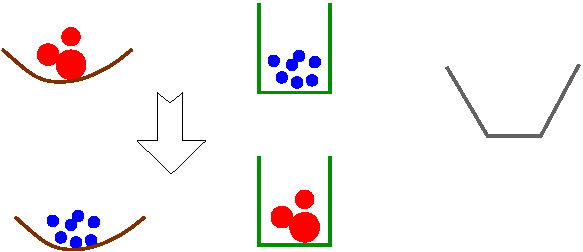
\includegraphics{Einterv_1.pdf}
 \caption{Intervertir les contenus de deux récipients}
 \label{fig:Einterv_1}
\end{figure}

Imaginons que l'on dispose de deux récipients contenant des objets. On veut les échanger. On sent bien qu'un troisième récipient est nécessaire et qu'il est alors facile de l'utiliser transitoirement.(Figure \ref{fig:Einterv_1})\newline
Dans la vraie vie, un récipient se \emph{vide} dans un autre ce qui n'est pas le cas avec des noms et des assignations. On pourrait imaginer que le récipient ne se vide pas mais que son contenu se duplique, ce n'est pas le cas non plus.

Considérons le code Python suivant
\begin{verbatim}
# initialisation
nom1 = "MickeydeTravers"
nom2 = "PetitsRondsBleus"
#Echange
nom3 = nom1
nom1 = nom2
nom2 = nom3
#Verification
print(nom1)
print(nom2)
\end{verbatim}
Après l'exécution de la première ligne du code ci dessus, quel est le type de l'objet désigné par \texttt{nom1}?
Quelle commande supplémentaire peut-on faire exécuter pour s'assurer qu'une assignation "ne vide pas" le nom placée à droite ?
Expliquez pourquoi le code suivant prouve que l'assignation ne copie pas les valeurs.
\begin{verbatim}
# initialisation
nom1 = ["disqueRouge1","disqueRouge2","disqueRouge3"]
nom2 = "PetitsRondsBleus"
print("valeurs initiales")
print(nom1)
print(nom2)

#Echange
nom3 = nom1
nom1 = nom2
nom2 = nom3

#Verification
print("échange")
print(nom1)
print(nom2)

print("modification")
print(nom3)
nom3.remove("disqueRouge2")
print(nom3)
print(nom2)
\end{verbatim}
Après l'exécution de la première ligne du code ci dessus, l'objet désigné par \texttt{nom1} est d'un type cité dans la partie 1. Principes; quel est ce type? Une propriété de ce type explique les résultats de l'exécution de ce code; laquelle? \newline
En utilisant une terminologie venant d'autres langages, on peut dire que l'assignation en Python se fait toujours \emph{par référence} et non \emph{par valeur}. C'est la raison fondamentale pour laquelle l'utilisation du mot \emph{nom} est préférable à celle de \emph{variable}.


\section{Premiers exercices}
\begin{enumerate}
  \item En utilisant les documents de cours distribués, expliquer sans l'exécuter ce que va faire et va afficher le code suivant:
\lstinputlisting[firstline=1, lastline=4]{exo_intro0_E.py}  
Vérifier qu'il se passe bien ce que vous aviez prévu en l'exécutant après l'avoir enregistré dans un fichier. Que se passe-t-il si on indente le \texttt{print(i)}?

  \item \'Ecrire deux programmes dont l'un exécutera 100 fois un bloc de code contenant un test et l'autre exécutera 49 fois un bloc contenant une incrémentation plus pertinente pour les problèmes suivants.
\begin{enumerate}
  \item Afficher tous les nombres impairs entre $0$ et $100$ par ordre croissant.
  \item Afficher tous les nombres pairs entre $0$ et $100$ par ordre décroissant.
\end{enumerate}

  \item La suite de Fibonacci est définie par
\begin{displaymath}
  f_0 = f_1 = 1, \hspace{1cm}\forall n \in \N,\; f_{n+2} = f_{n+1} + f_n
\end{displaymath}
Le calcul de ses termes doit se faire en utilisant la phrase invariante:
\begin{quote}
  \og $n$ désignant un entier, $f$ désigne $f_n$ et $ff$ désigne $f_{n+1}$\fg
\end{quote}
\'Ecrire deux programmes qui affichent les 20 premiers termes. Le premier programme utilisera les assignations multiples et pas le second. Modifier les programmes pour qu'ils n'affichent que le 20ème terme (c'est à dire $f_{19}$)

  \item En précisant la phrase invariante utilisée, écrire un programme qui affiche les 10 premiers termes de la suite récurrente définie par
\begin{displaymath}
  u_0 = 3, \hspace{0.5cm} \forall n \in \N, \;u_{n+1} = n + 2u_n
\end{displaymath}

  \item (à faire en dernier) \`A l'aide d'un programme utilisant 3 boucles "while" imbriquées, calculer le nombre de triplets $(x,y,z)$ d'entiers de $\llbracket 1, 10 \rrbracket$ tels que
  \begin{displaymath}
  1  \leq x < y < z \leq 10
  \end{displaymath}
Vérifiez en comparant avec une formule pour cette somme obtenue avec les techniques de calcul de somme.
\end{enumerate}

\end{document}